\documentclass[11pt]{article}

\usepackage[utf8]{inputenc}

\usepackage{amsmath}
\usepackage{graphicx}
\usepackage{enumerate}
\usepackage{hyperref}
\usepackage{subcaption}
\usepackage[all]{hypcap}
\usepackage{relsize}
\usepackage{caption}
\usepackage{array}
\usepackage[margin=1in, paperwidth=8.5in, paperheight=11in]{geometry}

\begin{document}

\title{Lab 3: Strain Guage}
\author{Wesley Soo-Hoo}
\maketitle

\begin{abstract}
    In this lab, a strain gauge was created using a Wheatstone bridge. Calibration measurements were taking using known masses and one unknown mass was measured, which will be calculated by using a linear regression of the calibration data.
\end{abstract}

\section{Hardware Setup}
Insert description of hardware Setup

\section{Data}
\subsection{Raw Data}
Insert table for raw data

\begin{table}[!ht]
	% the "!ht" will tell LaTeX to try and put the table here, and at the top of the next page if it doesn't fit here. Getting tables to show up where you want can be a pain
	
	\small                      % this makes the text in the table small
	\centering                  % this centers the table
	\caption{Raw Calibration Data} % always caption your tables!
	\label{tab:ninjahours}      % lets me reference the table (like with figures and equations) 
	
\begin{tabular}{m{1in}|m{1in}}
\textbf{Mass (g)}&	\textbf{Voltage (V)}\\ \hline
0&		0.001 \\
8.7&	0.051 \\
20.4&	0.092 \\
47.3&	0.16  \\
72.1&	0.25  \\
\end{tabular}

\end{table}

\begin{figure} [!ht]
	\centering
	
	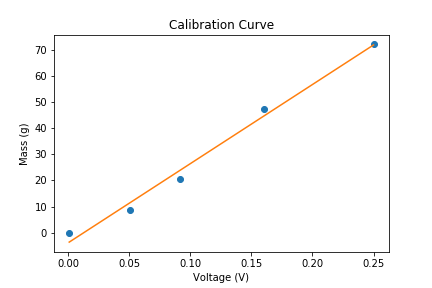
\includegraphics[width=0.75\textwidth]{../img/calibration.png}
	
	\captionsetup{margin={0.125\textwidth,0.125\textwidth}}
	\caption{\smaller{Graph of the calibration data including the line of best fit}}
	
	\label{fig:cal_graph}
\end{figure}

\subsection{Data Analysis}
Insert Data Analysis section here

\begin{equation}\label{eq:random}
    A_{out} = A_{in}\frac{B_2}{B_1}
\end{equation}
% \begin{equation} and \end{equation} are used to signify a numbered equation. Anything between these signifiers will be processed in math mode
% Notice how I also used \label{} within the equation to label it, so I can reference it easily throughout this document. By matching the text inside the curly brackets of the equation's \label{} and \ref{} in-line with text, LaTeX automatically inserts the correct equation number and creates a link between the number and the equation. As good practice, use "eq:" at the beginning of all equation labels

If you want to get fancy, you can align multiple lines of math, e.g.
\begin{align}
% to align multiple lines of math, use \begin{align} and \end{align}. Again, this signifies math mode
% the ampersand determines where the formula will be aligned
% using \begin{align*} and \end{align*} will get rid of the equation numbers
A^2 +B^2 &= C^2 \\
% carats will produce superscript, e.g. ^{this will be superscript}
\frac{C}{2D} &= E_1E_2E_3 \\
% remember to end each line in math mode with a \\, which forces a newline
% underscores will produce subscript, e.g. _{this will be subscript}
% \frac{numerator}{denominator} will produce a fraction
\left(\pi\frac{y+x^2}{\sqrt{\sin(\theta)}}\right) &= \text{something magical}
% putting \left and \right before parenthesis will make LaTeX automatically size them
% \text{this will be plaintext} will produce plaintext in mathmode
% to find how to use a symbol in mathmode, check out http://detexify.kirelabs.org/classify.html
% for more random math symbols in mathmode, just Google it
% WARNING: do not leave any blank lines in the source between the end of your math and \end{align}, or your document won't compile and you'll get funny errors about paragraphs ending
\end{align}

\section{Other Useful Features}
Another fun thing you can do in \LaTeX{} is lists.

\noindent For example, here are some random syntax tips:
\begin{itemize}
	\item To create quotes correctly, use backticks for the opening quote: ``this is in quotes"
    \item To write special characters as text, try adding a backslash in front of the character, e.g. \$
\end{itemize}

\noindent You can also create numbered lists. Here are some useful resources when trying to learn \LaTeX{}:
\begin{enumerate}
    \item To find the \LaTeX{} command for an unknown symbol, use \href{http://detexify.kirelabs.org/classify.html}{Detexify}!
	\item A great general resource is \href{https://www.sharelatex.com/learn/}{Share\LaTeX{}'s learning site}
	\item For more than you'd ever want to know about \LaTeX{}, check out the \href{http://en.wikibooks.org/wiki/LaTeX}{\LaTeX{} Wikibook}
\end{enumerate}

You can also make tables, although it's a bit of a pain. Two useful resources for tables in \LaTeX{} are \href{http://www.tablesgenerator.com/latex_tables}{tablesgenerator.com} and \href{https://www.sharelatex.com/learn/Tables}{the Share\LaTeX{} page on tables}. Your mileage may vary, but you can reference Table~\ref{tab:ninjahours} below as an example.

% TODO: UPDATE THIS OFFICE HOURS TABLE
% use \begin{table} and \end{table} to include a table
\begin{table}[!ht]
% the "!ht" will tell LaTeX to try and put the table here, and at the top of the next page if it doesn't fit here. Getting tables to show up where you want can be a pain

\small                      % this makes the text in the table small
\centering                  % this centers the table
\caption{NINJA Office Hours} % always caption your tables!
\label{tab:ninjahours}      % lets me reference the table (like with figures and equations) 

% this is where you create the actual table. As you can see, it's kind of a pain
% in this example, I'm using the array package to specify the column widths
\begin{tabular}{m{0.75in}|m{0.6in} m{0.6in} m{0.6in} m{0.6in} m{0.6in} m{0.6in} m{0.6in}}
&                   \textbf{Sun}&   \textbf{Mon}&   \textbf{Tue}&   \textbf{Wed}&   \textbf{Thu}&   \textbf{Fri}&   \textbf{Sat}\\ \hline
\textbf{6 - 7pm}&   Sophia&         Jeremy&         &               &               &               &               Franton\\
\textbf{7 - 8pm}&   Sophia&         Jeremy&         Vivien&         Annie&          Vivien&         &               Franton\\
\textbf{8 - 9pm}&   Emma&           Vivien&         &               Emma&           &               &               \\
\textbf{9 - 10pm}&  Emma&           Maggie&         Franton&        Emma&           Maggie&         &               \\
\textbf{10 - 11pm}& Annie&          Annie&          Prava&          Prava&          Prava&          &
\end{tabular}

\end{table}

\section{Finishing Remarks}
With the right packages, you can do anything from tables to subfigures to bibliographies. Like almost everything else, you can find out a lot about using \LaTeX by \href{http://lmgtfy.com/?q=how+to+LaTeX}{searching online}.

\end{document}